\documentclass[10pt]{article}
\usepackage{tikz}
\usepackage[margin=0cm]{geometry}
\pagestyle{empty}

\begin{document}

\vspace*{\fill}
\begin{center}
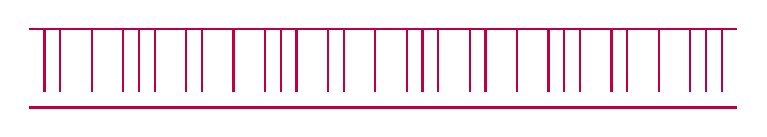
\begin{tikzpicture}[x=0.2cm, y=-0.2cm, thick, purple]
% North to South lines
    \draw (1,0) -- (1,4);
    \draw (2,0) -- (2,4);
    \draw (4,0) -- (4,4);
    \draw (6,0) -- (6,4);
    \draw (7,0) -- (7,4);
    \draw (8,0) -- (8,4);
    \draw (10,0) -- (10,4);
    \draw (11,0) -- (11,4);
    \draw (13,0) -- (13,4);
    \draw (15,0) -- (15,4);
    \draw (16,0) -- (16,4);
    \draw (17,0) -- (17,4);
    \draw (19,0) -- (19,4);
    \draw (20,0) -- (20,4);
    \draw (22,0) -- (22,4);
    \draw (24,0) -- (24,4);
    \draw (25,0) -- (25,4);
    \draw (26,0) -- (26,4);
    \draw (28,0) -- (28,4);
    \draw (29,0) -- (29,4);
    \draw (31,0) -- (31,4);
    \draw (33,0) -- (33,4);
    \draw (34,0) -- (34,4);
    \draw (35,0) -- (35,4);
    \draw (37,0) -- (37,4);
    \draw (38,0) -- (38,4);
    \draw (40,0) -- (40,4);
    \draw (42,0) -- (42,4);
    \draw (43,0) -- (43,4);
    \draw (44,0) -- (44,4);
% North-West to South-East lines
% West to East lines
    \draw (0,0) -- (45,0);
    \draw (0,5) -- (45,5);
% South-West to North-East lines
\end{tikzpicture}
\end{center}
\vspace*{\fill}

\end{document}
